My prototype is called Desktop (see Figure \ref{fig:desktop}). Expanding on the initial game structure we formed 
our ideas around, my prototype adds the ability for users to declare variables and data structures. The idea 
is that by making the user responsible for managing these resources directly it will help reinforce the concepts 
associated with each element.\\

\begin{figure}[!hb]
	\centering
	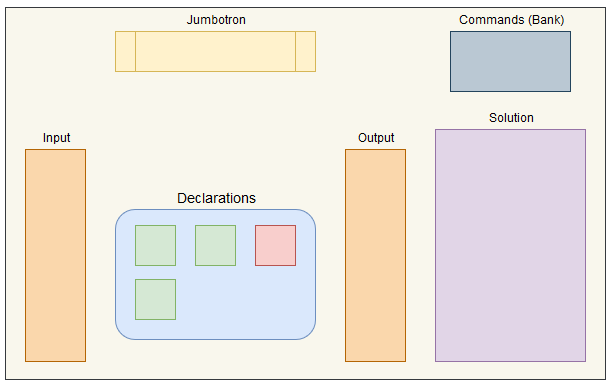
\includegraphics{desktop}
	\caption{Sample layout of the basic level design. An actor will move around the field and carry out the commands selected by the user in the Solution area.}
	\label{fig:desktop}
\end{figure}

\textbf{\textit{Setting}}\\
The playing field of Desktop takes place on top of a desk. A small figurine on the desk comes to life at the start 
of the game and moves around the desktop during gameplay. Each level of the game is a puzzle designed to 
test the user on their skills with computational thinking. Tutorial style levels, which occur whenever a new 
command or data structure is introduced, will feature a short to-do list for the player to complete to ensure they
 understand the concept before they are required to use it to solve a puzzle.\\

\textbf{\textit{Elements}}\\
\textbf{Input:}
The input trough will feature a queue of pieces of data that the user will need to manipulate in order to solve 
the puzzle. Data can only be picked up one at a time, and only the topmost piece of data can be selected - the 
player cannot pick up an arbitrary piece from the queue. The values of the data will be randomly generated 
when each level is loaded, and puzzles must be dynamic to handle any number of data elements with any value. 
Data cannot be placed back into the queue once it has been removed. The style of the input trough is to be 
determined.\\

\textbf{Output:}
The output trough is the area where the manipulated pieces of data should be placed in the expected order 
for a correct solution. As an element is added to this queue, it will push the rest of the elements down so that 
the first element is always on the bottom and the most recently added element is always on top. Data cannot 
be retrieved from the queue once it has been placed. The style of the output trough is to be determined.\\

\textbf{Declarations:}
This is the designated area for players to place their declared variables and data structures. These items cannot 
be used in the commands within the solution unless they have been placed here first. The variables and data 
structures will be stored in the commands bank, and players will drag them to the declarations area in order to 
declare them. When the items are dropped here they will snap into the grid. There is a limited amount of space 
available for the player to utilize, so more intricate puzzles will require the player to manage their declarations 
more closely. The declarations area will be styled after a notebook.\\

\textbf{Commands:}
This is a storage area. It will consist of a listed bank of commands -- as well as the variable and data structure 
elements -- currently available to the user. The commands will appear as small rectangular cards and will be 
manipulated with drag-and-drop controls. The variable and data structure elements will be square shaped to 
make them easily differentiable from the commands. For more information on each of the structures and 
commands, see their respective sections below. The commands area will be styled after a stacked document 
sorter, with loose plans for the player to select which “level” of the sorter they are pulling from - commands 
or data structures. Further separating these two components will help keep the concepts discreet from one 
another.\\

\textbf{Solution:}
This is the area where the player will drag-and-drop their commands in order to build a solution to the puzzle. 
If the solution length exceeds the size of the box, a scroll bar will pop up so that users can navigate through 
their solution. The bottom of this box will have a fixed panel with debugging buttons and a button to run the 
current solution. While a solution is running, an indicator will pop up in the solution box and point at which 
command is currently being carried out by the figurine. The debugging buttons will feature a step button that 
executes only the next line of code, a back button that undoes the last line of code executed, and a stop button 
that will halt the current running solution. Players will be able to rearrange commands within the solution box by 
dragging them to different places within the solution. Similar to how structures will snap to a grid within the 
declarations box, commands will align within the solution box in sequence. The alignment will be dynamic 
whenever a command is being drug through the current sequence of commands so that users can see precisely 
where any inserted commands will be placed. Commands that are inside of an if block will be indented to more 
clearly show the user what is part of the conditional logic. When if blocks are open, the subsequent commands 
will automatically be aligned with the indentation until the user places a command flushed left. This alignment will 
also be dynamic, where users can drag commands right or left to either include them in the block or mark the 
end of the block. The command area will be styled after a yellow legal pad.\\

\textbf{Figurine:}
The figurine will be a small animated character that moves around the desktop, carrying out the commands that 
the user has selected in the solution box. The user will only be able to manipulate the data in the puzzle through 
the actions of the figurine, which are subsequently controlled by the sequence of commands in the solution box. 
The animations of the figurine will assist in conveying how the data is being manipulated by the commands, as 
well as clearly displaying how the sequence of commands in the solution is working to solve the problem. The 
figurine will become visibly upset when a solution fails to find the correct solution, and will cease their actions 
whenever a program halting error is encountered. They will also be the source of providing information to the 
player. If the player clicks on the figurine while they are in a halted state, the figurine can provide feedback to 
the player. When errors halt the figurine, it can inform players on the type of error. If the figurine is at a natural 
halt (ie, the solution finished running but didn’t find the correct solution), it can provide tips and hints to the 
player that can help clarify the goals of the current puzzle. Additionally, this character will be the method of 
delivering newly acquired commands and structures to the player. The exact design of the figurine is to be 
determined.\\

\textbf{Jumbotron:}
The purpose of the Jumbotron is to provide an additional level of clarity to the user. Its sole purpose is to 
essentially broadcast which command the figurine is currently executing. This helps address the issue with 
players only paying attention to the character when running their solutions and not watching the sequence 
being followed within the solution box. The Jumbotron will be styled after a desktop digital clock displaying 
the current command instead of the time, and will flash to indicate a change of command.\\

\textbf{To-Do List:}
The to-do list is located in the upper left hand corner of the desk, and will only become active when the user 
is in a tutorial level. Its purpose is to list the specific tasks that the player needs to accomplish with their new 
command or data structure to demonstrate their understanding of it. Check boxes on the to-do list will automatically 
get ticked off once the task is completed, and players will not be allowed to advance to the next level until all 
tasks on the list are satisfied. During this time, the play area becomes an open play arena, with endless input for 
the player to manipulate. Solutions can be run as normal, but there is no expected correct solution for these levels. 
The player is allowed to freely manipulate data however they want in order to test out their new tools, as well as play 
around with all of the other commands and structures currently available to them. Once all of the items on the to-do 
list are achieved, a button next to the to-do list illuminates and they can choose to move forward to the next puzzle 
whenever they are ready to do so. The to-do list will be styled after a post-it note.\\

\textbf{\textit{Structures}}\\
For all of the structures available to the user, they are not required to maintain the storage of data within the 
structure. Everything that is related to structure and storage will be handled on the back end. This allows the 
user to concentrate solely on the concept of the structure.\\

\textbf{Variable:}
The variable structure can hold a single piece of data. If new data is stored in the variable, the previous value 
being held is lost. Data can be copied from or removed from the variable. The variable will be visualized as a 
single square.\\

\textbf{Heap:}
The player selects if they want a MinHeap or MaxHeap when declaring the heap structure. Multiple pieces of 
data can be stored in a heap. The player is only able to copy or remove the top element from the heap, either 
the min or max depending on which type of heap they are using. When new elements are added to the heap, 
it shakes on screen as it sorts the data. The heap will be visualized as a stack of squares, but only the top 
element will be visible.\\

\textbf{Stack:}
Multiple pieces of data can be stored in a stack. The player can only remove the topmost element from the 
stack. The stack will be visualized as a stack of boxes, but only the top element will be visible. When new 
elements are added to the stack, a new box appears on the top with the most recently added element. Once 
the number of elements in the stack is five additional boxes that are added don’t cause the stack to visually 
expand, but the data will be maintained for any number of elements in the stack.\\

\textbf{Queue:}
Multiple pieces of data can be stored in a queue. The player can only remove the first element from the queue. 
The queue will be visualized as a stack of boxes, but only the first element will be visible. When new elements 
are added to the stack, a new box is slid underneath the current stack, and only the first element of the queue 
is visible. Once the number of elements in the queue is five, additional boxes that are added don’t cause the 
queue to visually expand, but the data will be maintained for any number of elements in the queue.\\

\textbf{\textit{Commands}}\\
Many commands within Desktop have blank fields that the user needs to fill in. Whenever one of these commands
 is first played in the solution box, the available items on the board that can be used to fill that blank are outlined 
with a bright glow, and the player must click on the item they want to use in that blank. The user can also change 
the designated item by clicking on the command itself within the solution box, which will cause the items to illuminate 
again so the user can change the selected item. The applicable items are input and output by default but can also 
include variables and data structures that have been declared. The piece of data that will be manipulated is described 
within the relevant section for that item. If a command is not able to be used on one of these items, it will be explicitly 
stated for that command.\\

\textbf{Pick Up (blank):}
This command will cause the figurine to pick up the applicable data element from the specified item. Any data currently 
being held by the figurine is lost. This command cannot be used on output.\\

\textbf{Put Down (blank):}
This command will cause the figurine to put down the data they are currently holding in the specified item. The figurines 
hands will be empty after this executes. This command cannot be used on input.\\

\textbf{Copy To (blank):}
This command will cause the figurine to make a copy of the data they are currently holding and place the copy in the 
specified item. The figurine will still be holding the original data after this executes. This command cannot be used on 
input or output.\\

\textbf{Copy From (blank):}
This command will cause the figurine to make a copy of the applicable data element from the specified item and hold 
the copy in their hands. Any data held by the figurine before this executes is lost. There are no errors associated with 
this command. This command cannot be used on input or output.\\

\textbf{Jump:}
This command causes the sequence of execution of commands to jump to the specified command. When it is played, 
the user has to drag an arrow attached to the jump command card and hook it into another instruction in the command 
box. There are no errors associated with this command.\\

\textbf{Add:}
This command will have the figurine pick up the applicable data element from the selected item and add it to the data they 
are currently holding. If this command executes when the figurines’ hands are empty, it causes an error. This command 
can only be used on variables.\\

\textbf{Subtract:}
This command will have the figurine pick up the applicable data element from the selected item and subtract it from the 
data they are currently holding. If this command executes when the figurines’ hands are empty, it causes an error. This 
command can only be used on variables.\\

Using if commands in Desktop causes subsequent commands in the solution box to be indented one level to show 
they are part of the conditional block. Users have to drag commands to the left to end the indentation and the conditional 
block.\\

\textbf{If Less Than (blank):}
This command will have the figurine compare the data in their hands to the applicable data element in the specified item. 
If the value of the data they are holding is less than the targeted data, the commands within the if block will be executed. 
Otherwise, the conditional block will be skipped. If this command executes when the figurines’ hands are empty, it causes 
an error. This command cannot be used on input or output.\\

\textbf{If Greater Than (blank):}
This command will have the figurine compare the data in their hands to the applicable data element in the specified item. If 
the value of the data they are holding is greater than the targeted data, the commands within the if block will be executed. 
Otherwise, the conditional block will be skipped. If this command executes when the figurines’ hands are empty, it causes 
an error. This command cannot be used on input or output.\\

\textbf{If Equal To (blank):}
This command will have the figurine compare the data in their hands to the applicable data element in the specified item. If 
the value of the data they are holding is equal to the targeted data, the commands within the if block will be executed. 
Otherwise, the conditional block will be skipped. If this command executes when the figurines’ hands are empty, it causes 
an error. This command cannot be used on input or output.\\

\textbf{\textit{Needed Improvements}}\\
At the time of prototyping, Desktop does not have a way to check whether or not an empty condition might occur. This 
is problematic because we need some form of verification that a specified item is empty, like the input or a particular data 
structure. This missing piece will help bring together the type of algorithmic design and computational thinking that Desktop 
aims to convey to users.\\

\newpage